\chapter{Конструкторский раздел}
В данном разделе представлены требования к разрабатываемому ПО, схемы алгоритмов умножения матриц, а также оптимизация алгоритма Винограда.

\section{Требования к ПО}

К программе предъявляется ряд требований:
\begin{itemize}
	\item корректное умножение матриц размером до $[N \times N]$, где $N\in[0:2000]$;
	\item при матрицах неправильных размеров программа не должна аварийно завершаться.
\end{itemize}

\section{Схемы алгоритмов}
Ниже представлены схемы следующих алгоритмов сортировки:
\begin{itemize}
	\item схема классического алгоритма умножения матриц (Рисунок \ref{img:m_std});
	\item схема алгоритма Винограда (рисунки \ref{img:m_winograd} - \ref{img:m_winograd2});
\end{itemize}

\section{Оптимизация алгоритма Винограда}
В рамках данной лабораторной работы было предложено 3 оптимизации:
\begin{enumerate}
	\item избавление от деления в условии цикла;
	\item замена двух операций $+$ и $=$ на одну $+=$ (это нам позволяет сделать язык программирования);
	\item внесение обработки нечётных размеров векторов в цикл заполнения ячеек матрицы результата.
\end{enumerate}

\begin{figure}
	\center{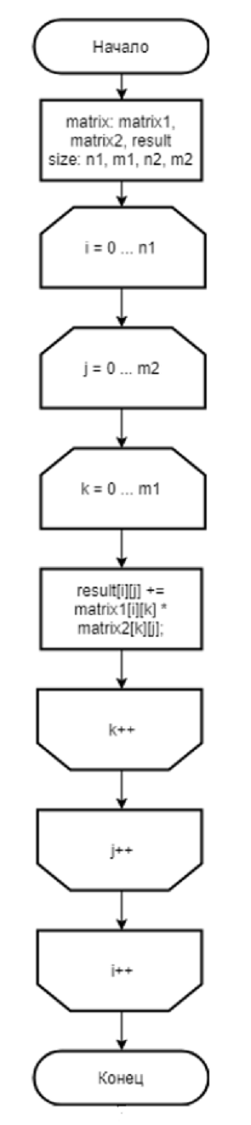
\includegraphics[width=0.3\linewidth]{inc/img/m_std}}
	\caption{Схема классического алгоритма умножения матриц}
\end{figure}

\begin{figure}
	\center{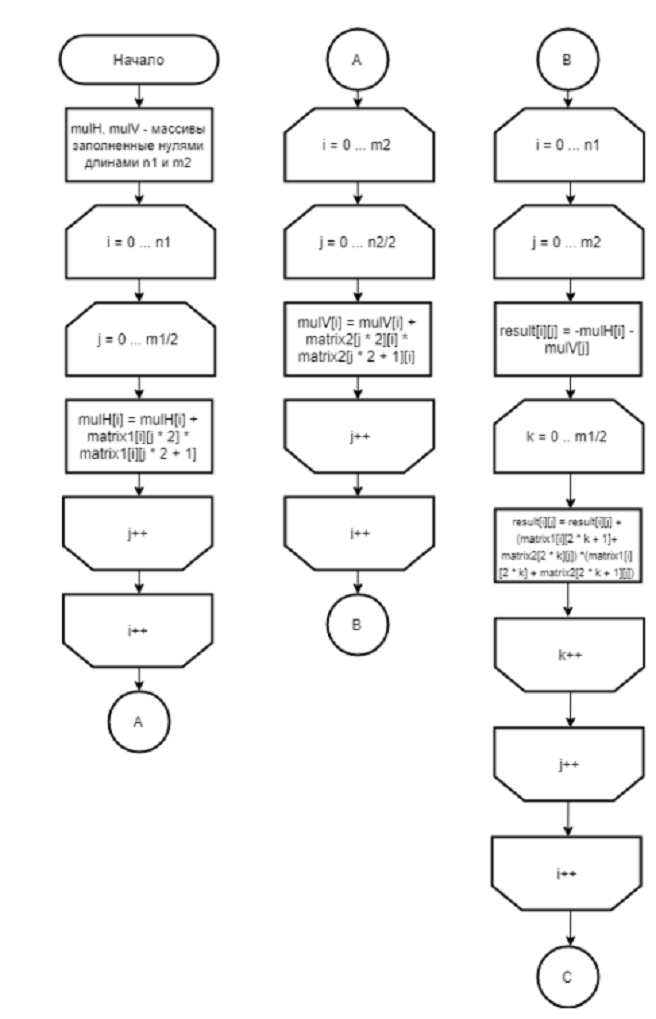
\includegraphics[width=0.9\linewidth]{inc/img/m_winograd}}
	\caption{Схема алгоритма Винограда}
\end{figure}

\begin{figure}
	\center{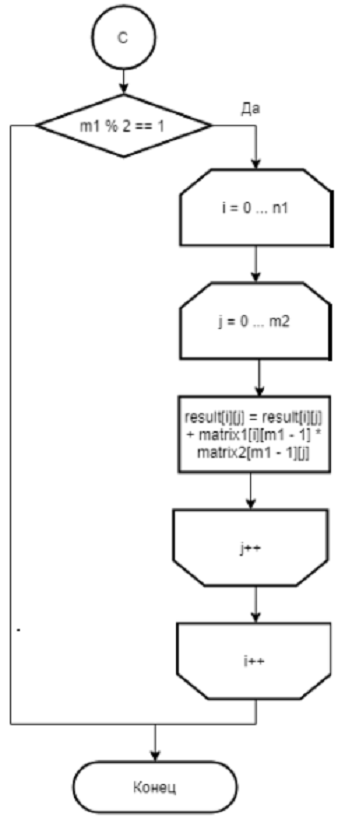
\includegraphics[width=0.6\linewidth]{inc/img/m_winograd2}}
	\caption{Схема алгоритма Винограда (продолжение)}
\end{figure}

\newpage
\section{Вывод}
В данном разделе были представлены требования к разрабатываемому ПО, произведена модификация алгоритма Винограда и разработаны схемы алгоритмов умножения матриц.